\usetikzlibrary{shadows}
\usetikzlibrary{arrows}
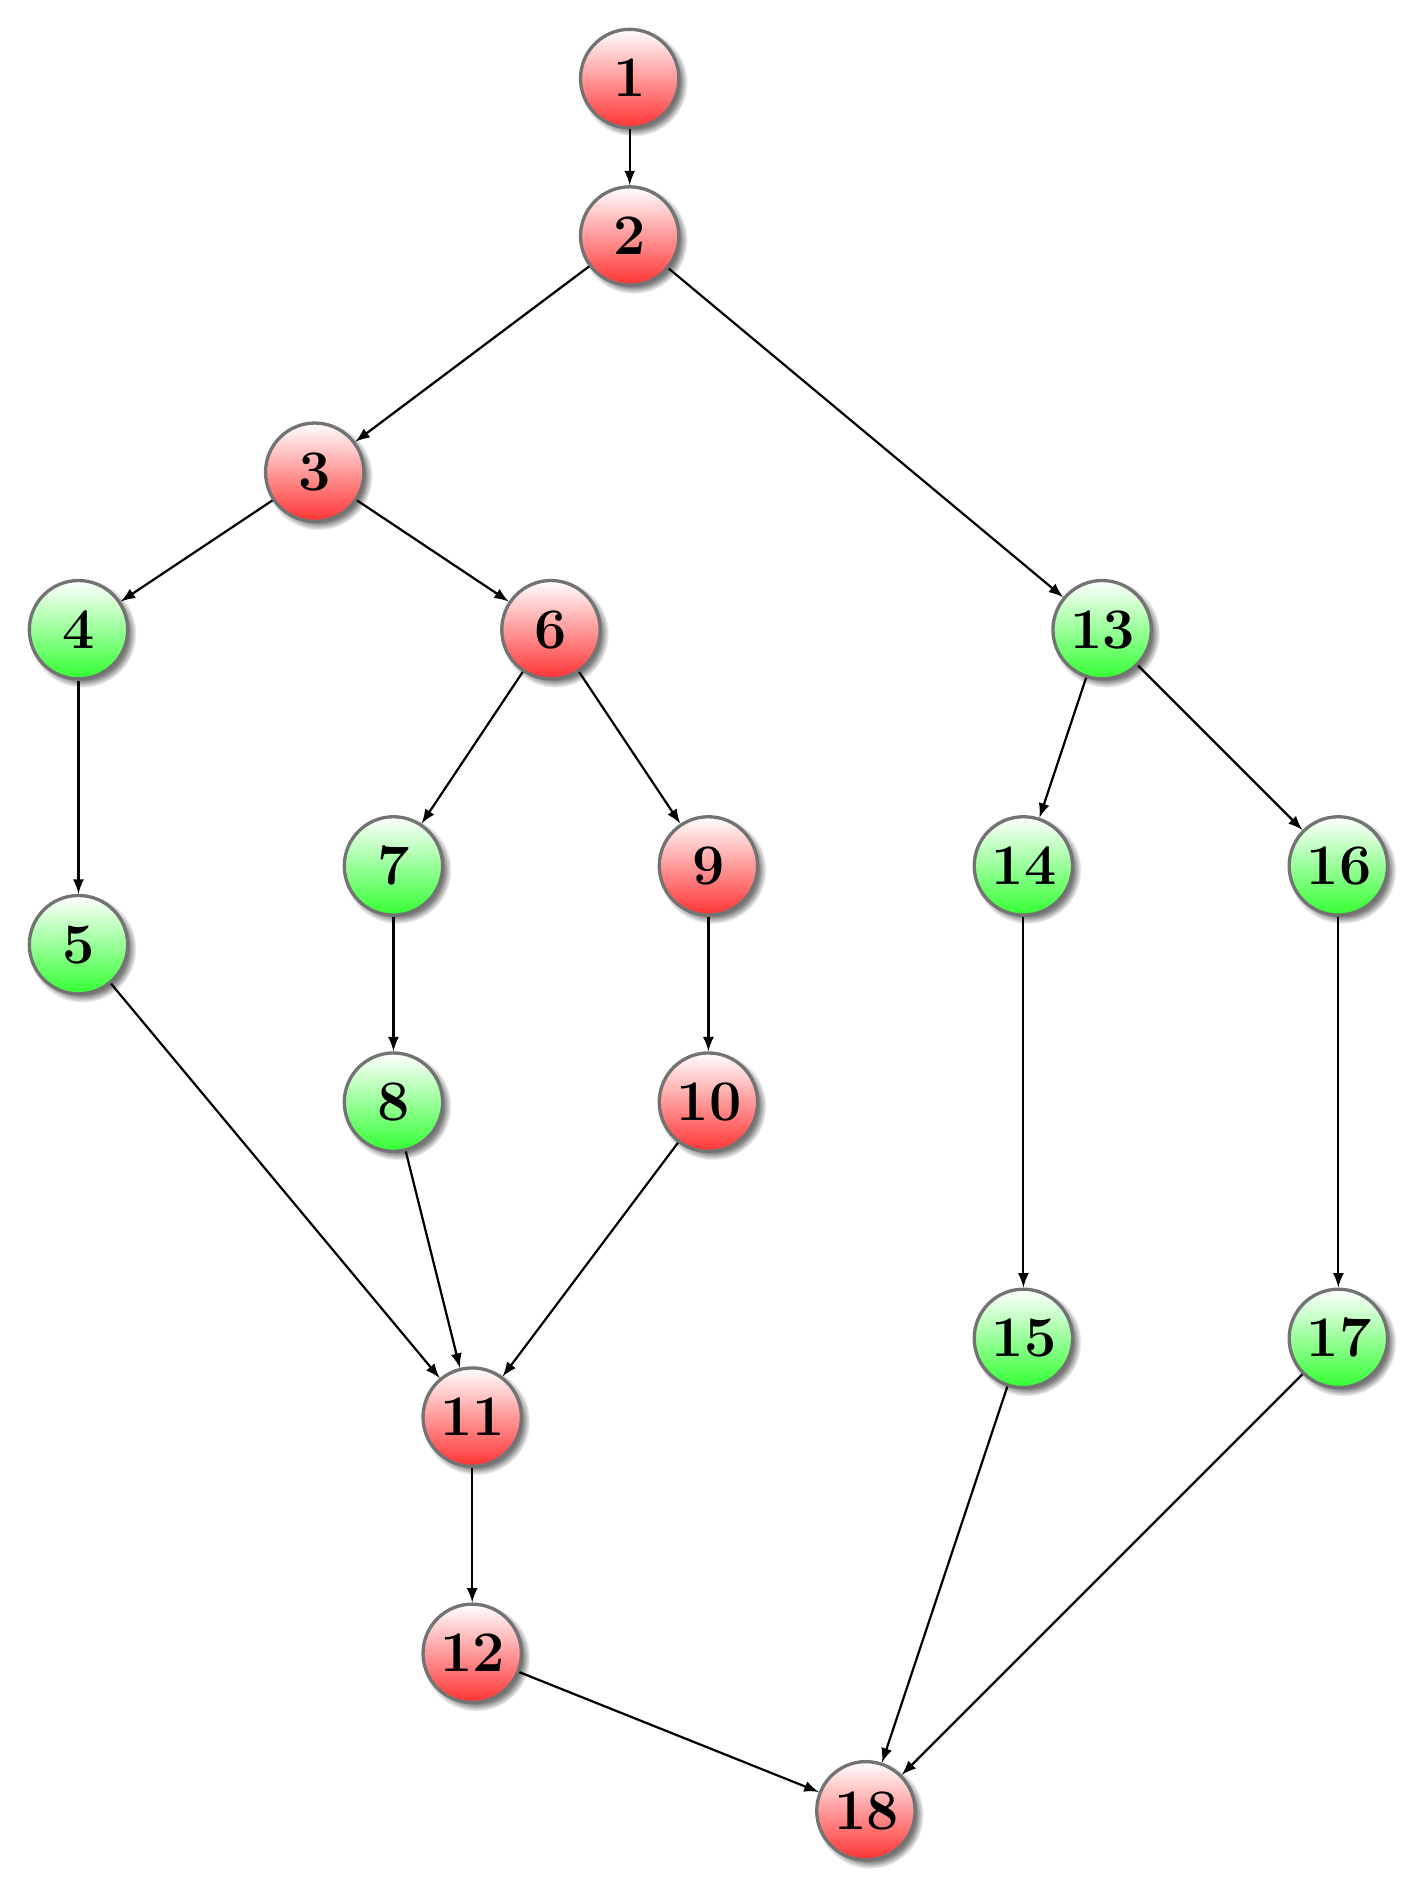
\begin{tikzpicture}

\node [ font={\huge\bfseries}, shape=circle, minimum size=0.8cm, circular drop shadow, text=black, very thick, draw=black!55, top color=white,bottom color=red!80, text width=0.8cm, align=center] (v1) at (-1,5) {1};
\node [ font={\huge\bfseries}, shape=circle, minimum size=0.8cm, circular drop shadow, text=black, very thick, draw=black!55, top color=white,bottom color=red!80, text width=0.8cm, align=center] (v2) at (-1,3) {2};
\node [ font={\huge\bfseries}, shape=circle, minimum size=0.8cm, circular drop shadow, text=black, very thick, draw=black!55, top color=white,bottom color=red!80, text width=0.8cm, align=center] (v3) at (-5,0) {3};
\node [ font={\huge\bfseries}, shape=circle, minimum size=0.8cm, circular drop shadow, text=black, very thick, draw=black!55, top color=white,bottom color=green!80, text width=0.8cm, align=center] (v5) at (-8,-2) {4};
\node [ font={\huge\bfseries}, shape=circle, minimum size=0.8cm, circular drop shadow, text=black, very thick, draw=black!55, top color=white,bottom color=red!80, text width=0.8cm, align=center] (v8) at (-2,-2) {6};
\node [ font={\huge\bfseries}, shape=circle, minimum size=0.8cm, circular drop shadow, text=black, very thick, draw=black!55, top color=white,bottom color=green!80, text width=0.8cm, align=center] (v4) at (5,-2) {13};
\node [ font={\huge\bfseries}, shape=circle, minimum size=0.8cm, circular drop shadow, text=black, very thick, draw=black!55, top color=white,bottom color=green!80, text width=0.8cm, align=center] (v6) at (-8,-6) {5};
\node [ font={\huge\bfseries}, shape=circle, minimum size=0.8cm, circular drop shadow, text=black, very thick, draw=black!55, top color=white,bottom color=green!80, text width=0.8cm, align=center] (v9) at (-4,-5) {7};
\node [ font={\huge\bfseries}, shape=circle, minimum size=0.8cm, circular drop shadow, text=black, very thick, draw=black!55, top color=white,bottom color=green!80, text width=0.8cm, align=center] (v12) at (-4,-8) {8};
\node [ font={\huge\bfseries}, shape=circle, minimum size=0.8cm, circular drop shadow, text=black, very thick, draw=black!55, top color=white,bottom color=red!80, text width=0.8cm, align=center] (v10) at (0,-5) {9};
\node [ font={\huge\bfseries}, shape=circle, minimum size=0.8cm, circular drop shadow, text=black, very thick, draw=black!55, top color=white,bottom color=red!80, text width=0.8cm, align=center] (v11) at (0,-8) {10};
\node [ font={\huge\bfseries}, shape=circle, minimum size=0.8cm, circular drop shadow, text=black, very thick, draw=black!55, top color=white,bottom color=red!80, text width=0.8cm, align=center] (v7) at (-3,-12) {11};
\node [ font={\huge\bfseries}, shape=circle, minimum size=0.8cm, circular drop shadow, text=black, very thick, draw=black!55, top color=white,bottom color=red!80, text width=0.8cm, align=center] (v13) at (-3,-15) {12};
\node [ font={\huge\bfseries}, shape=circle, minimum size=0.8cm, circular drop shadow, text=black, very thick, draw=black!55, top color=white,bottom color=green!80, text width=0.8cm, align=center] (v15) at (4,-5) {14};
\node [ font={\huge\bfseries}, shape=circle, minimum size=0.8cm, circular drop shadow, text=black, very thick, draw=black!55, top color=white,bottom color=green!80, text width=0.8cm, align=center] (v16) at (4,-11) {15};
\node [ font={\huge\bfseries}, shape=circle, minimum size=0.8cm, circular drop shadow, text=black, very thick, draw=black!55, top color=white,bottom color=green!80, text width=0.8cm, align=center] (v17) at (8,-5) {16};
\node [ font={\huge\bfseries}, shape=circle, minimum size=0.8cm, circular drop shadow, text=black, very thick, draw=black!55, top color=white,bottom color=green!80, text width=0.8cm, align=center] (v18) at (8,-11) {17};
\node [ font={\huge\bfseries}, shape=circle, minimum size=0.8cm, circular drop shadow, text=black, very thick, draw=black!55, top color=white,bottom color=red!80, text width=0.8cm, align=center] (v14) at (2,-17) {18};
\draw [-latex,thick] (v1) edge (v2);
\draw [-latex,thick] (v2) edge (v3);
\draw [-latex,thick] (v2) edge (v4);
\draw [-latex,thick] (v3) edge (v5);
\draw [-latex,thick] (v5) edge (v6);
\draw [-latex,thick] (v6) edge (v7);
\draw [-latex,thick] (v3) edge (v8);
\draw [-latex,thick] (v8) edge (v9);
\draw [-latex,thick] (v8) edge (v10);
\draw [-latex,thick] (v10) edge (v11);
\draw [-latex,thick] (v9) edge (v12);
\draw [-latex,thick] (v12) edge (v7);
\draw [-latex,thick] (v11) edge (v7);
\draw [-latex,thick] (v7) edge (v13);
\draw [-latex,thick] (v13) edge (v14);
\draw [-latex,thick] (v4) edge (v15);
\draw [-latex,thick] (v15) edge (v16);
\draw [-latex,thick] (v4) edge (v17);
\draw [-latex,thick] (v17) edge (v18);
\draw [-latex,thick] (v18) edge (v14);
\draw [-latex,thick] (v16) edge (v14);
\end{tikzpicture}